\documentclass{beamer}
\usetheme{Warsaw}  %% Themenwahl

\usepackage{amsmath,amssymb,amsthm}
\usepackage{tikz}
\usetikzlibrary{arrows,shapes,positioning,automata}
\usepackage{listings}
\usepackage{xspace}

\title{Geometric Nontermination Arguments}
\author{Timo Bergerbusch}
\date{\today}


\lstset{
	backgroundcolor=\color{white},	% choose the background color
	basicstyle=\ttfamily,			% the size of the fonts that are used for the code
	breakatwhitespace=false,		% sets if automatic breaks should only happen at whitespace
	breaklines=true,				% sets automatic line breaking
	captionpos=b,					% sets the caption-position to bottom
	commentstyle=\color{green!60!black},% comment style
	deletekeywords={...},			% if you want to delete keywords from the given language
	escapeinside={\%*}{*)},			% if you want to add LaTeX within your code
	frame=none,					% adds a frame around the code
	keepspaces=false,				% keeps spaces in text, useful for keeping indentation of code
	% (possibly needs columns=flexible)
	keywordstyle=\color{blue},		% keyword style
	lineskip=0.1pt,
	%linewidth=0.7\linewidth,
	frame=lines,
	morekeywords={*,...},			% if you want to add more keywords to the set
	numbers=left,				% where to put the line-numbers; possible values are (none, left, right)
	numbersep=5pt,				% how far the line-numbers are from the code
	numberstyle=\tiny\color{gray},		% the style that is used for the line-numbers
	rulecolor=\color{black},			% if not set, the frame-color may change on line-breaks within not-black text
	showspaces=false,				% show spaces using underscores; overrides 'showstringspaces'
	showstringspaces=false,			% underline spaces within strings only
	showtabs=false,				% show tabs within strings adding particular underscores
	stepnumber=1,				% the step between two line-numbers. If it's 1, each line will be numbered
	stringstyle=\color{mymauve},		% string literal style
	tabsize=2,					% sets default tabsize to 2 spaces
	%title=\lstname	,				% show the filename of files included with \lstinputlisting; also try caption instead of title
} 

\tikzstyle{arrow} = [->]
\tikzstyle{thickarrow}=[arrow, thick]
\tikzstyle{dashedarrow} = [thickarrow, >=stealth, dashed, line width = 1pt ]
\tikzstyle{stdNode} = [shape = rectangle, draw, rounded corners]
\tikzstyle{aproveNode} = [shape = rectangle, draw, rounded corners, minimum width = 2cm]
\tikzstyle{objDia}=[rectangle, draw=black, rounded corners, text centered, anchor=north, rectangle split, rectangle split parts=2]
\tikzstyle{class}=[rectangle, draw=black, rounded corners, text centered, anchor=north, rectangle split, rectangle split parts=3]
\tikzstyle{explNode} = [align = center, minimum height = 10pt,	font = \bfseries, fill= green!20]
\tikzstyle{considered}=[thickarrow, color = blue]
\tikzstyle{neglected} = [thickarrow, color = red]
\tikzstyle{query} = [thickarrow, color = green!50!black]

\newcommand{\code}[1]{\textit{#1}}
\newcommand{\tool}[1]{\textsf{#1}}
\newcommand{\aprove}{\tool{AProVE}\xspace}
\newcommand{\HRule}[1]{\rule{\linewidth}{#1}}
\newcommand{\stem}{\textit{STEM}\xspace}
\newcommand{\loopt}{\textit{LOOP}\xspace}
\newcommand{\guardmatrix}{\textit{Guard Matrix}\xspace}
\newcommand{\guardconstants}{\textit{Guard Constants}\xspace}
\newcommand{\updatematrix}{\textit{Update Matrix}\xspace}
\newcommand{\updateconstants}{\textit{Update Constants}\xspace}
\newcommand{\iterationmatrix}{\textit{Iteration Matrix}\xspace}
\newcommand{\iterationconstants}{\textit{Iteration Constants}\xspace}
\newcommand{\startterm}{\textit{start term}\xspace}
\newcommand{\gna}{\textit{geometric nontermination argument}\xspace}
\newcommand{\gnanal}{\textit{geometric nontermination analysis}\xspace}
\newcommand{\rpntree}{\textit{Reverse Polish Notation Tree}\xspace}
\newcommand{\smtfactory}{\code{SMTFactory}\xspace}
\newcommand{\its}{\tool{int-TRS}\xspace}
\newcommand{\llvm}{\tool{llvm}\xspace}
\newcommand{\nonterm}{\textit{non-termination}\xspace}
\newcommand{\seg}{\textit{Symbolic Execution Graph}\xspace}
\newcommand{\stdLinInt}{standard linear integer form\xspace}
\newcommand{\stdG}{standard guard form\xspace}
\newcommand{\strG}{strict guard form\xspace}
\newcommand{\solver}{\textit{SMT}-\textit{solver}\xspace}
\newcommand{\domc}{\textit{Domain Criteria}\xspace}
\newcommand{\initc}{\textit{Initiation Criteria}\xspace}
\newcommand{\pointc}{\textit{Point Criteria}\xspace}
\newcommand{\rayc}{\textit{Ray Criteria}\xspace}
\newcommand{\addass}{\textit{Additional assertion}\xspace}
\newcommand{\qfnia}{\textit{quantifier free non-linear integer arithmetic}\xspace}
\newcommand{\lasso}{\tool{lasso}\xspace}

\newenvironment{variableblock}[3]{%
	\setbeamercolor{block body}{#2}
	\setbeamercolor{block title}{#3}
	\begin{block}{#1}}{\end{block}}

\begin{document}
\maketitle
\frame{\tableofcontents[currentsection]}

\section{Einleitung}
\frame{\tableofcontents[currentsection]}

\begin{frame} %%Eine Folie
  \frametitle{Einleitung und Motivation}
  \begin{itemize}
  	\item Verbreitung von Software
  	\item Automatische Entwicklungsunterst\"utzung $\Rightarrow$\red{Halte Problem}
  	\item \aprove\newline
	  	\begin{figure}[H]
	  		\centering
		  	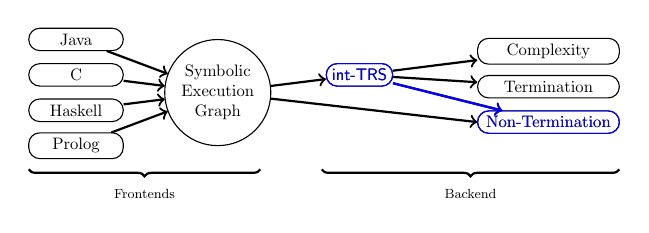
\begin{tikzpicture}[scale=0.6, every node/.style={scale=0.6}]
			  	\node[aproveNode] at (0,0) (java) {Java};
			  	\node[aproveNode]at (0,-.75) (c) {C};
			  	\node[aproveNode] at (0,-1.5) (haskell) {Haskell};
			  	\node[aproveNode] at (0,-2.25) (prolog) {Prolog};
			  	\node[shape = circle, draw,align = center] at (3, -1.125) (seg) {Symbolic\\ Execution\\ Graph};
			  	\node<1>[stdNode] at (6,-.75) (its) {\its};			  	
			  	\node<2>[stdNode, color = blue] at (6,-.75) (its) {\its};
			  	\node[stdNode, minimum width = 3cm] at (10,-.25) (comp) {Complexity};
			  	\node[stdNode, minimum width = 3cm] at (10,-1) (term) {Termination};
			  	\node<1>[stdNode, minimum width = 3cm] at (10,-1.75) (nterm) {Non-Termination};
			  	\node<2>[stdNode, minimum width = 3cm, color = blue] at (10,-1.75) (nterm) {Non-Termination};
			  	
			  	\draw[thickarrow] (java) edge (seg);
			  	\draw[thickarrow] (c) edge (seg);
			  	\draw[thickarrow] (haskell) edge (seg);
			  	\draw[thickarrow] (prolog) edge (seg);
			  	
			  	\draw[thickarrow] (seg) edge (its);
			  	\draw[thickarrow] (seg) edge (nterm.west);
			  	
			  	\draw[thickarrow] (its) edge (term);
			  	\draw[thickarrow] (its) edge (comp);
			  	\draw<1>[thickarrow] (its) edge (nterm);
			  	\draw<2>[thickarrow, color = blue] (its) edge (nterm);
			  	
			  	\draw [thick,decoration={brace,mirror},decorate] (-1,-2.75) -- (3.9,-2.75) 
			  	node [pos=0.5,anchor=north,yshift=-0.3cm] {\footnotesize Frontends}; 
			  	
			  	\draw [thick,decoration={brace,mirror},decorate] (5.2,-2.75) -- (11.5,-2.75) 
			  	node [pos=0.5,anchor=north,yshift=-0.3cm] {\footnotesize Backend}; 
		  	\end{tikzpicture}
		\end{figure}
	
  \end{itemize}
\end{frame}

%TODO: mention its derivation
\section{Example}

\begin{frame}[fragile] %%Eine Folie
  \frametitle{Example \tool{C}-program} %%Folientitel
  \begin{columns}
  	\begin{column}{6cm}
  		\begin{lstlisting}[language = java,escapechar = !]
int main(){
  		
	int a;!\tikz[remember picture] \node [] (a) {};!
	int b=1;!\tikz[remember picture] \node [] (b) {};!
  		
	while(a+b>=4){! \tikz[remember picture] \node [] (c) {}; !
    a=3*a+b;!\tikz[remember picture] \node [] (d) {}; !
    b=2*b-5;!\tikz[remember picture] \node [] (e) {}; !
	}
}		
  		\end{lstlisting}
%  		\begin{tikzpicture}[remember picture, overlay, 
%  		every edge/.append style = {dashedarrow},
%  		every node/.append style = {explNode},
%  		text width = 2cm ]
%  		\node[above right = .2cm and 2.5 cm of a] (A) {the \textit{STEM}};
%  		\draw[rounded corners=5pt] (A.west) edge (a.east);
%  		\draw (A.west) edge (b.east);
%  		
%  		\node[below = 1.5cm of A] (B) {the guard};
%  		\draw (B.west) edge (c.east);
%  		
%  		\node[below = .8cm of B] (C) {the linear update};
%  		\draw (C.west) edge (d.east);
%  		\draw (C.west) edge (e.east);
%  		\end{tikzpicture}
  	\end{column}
	\begin{column}{5cm}
		\begin{itemize}			
			\item very basic \tool{C}-program
			\item does it terminate?
			\item[] $\Rightarrow$ \color{red}No!\color{black}
			\item[] how can we prove this?
		\end{itemize}
	\end{column}
  \end{columns}
\end{frame}
\section{N{\"o}tiges Vorwissen}

\subsection{Integer-Transitionssysteme (ITS) }
\frame{\tableofcontents[currentsection]}
\begin{frame}[fragile] %%Eine Folie
	\frametitle{Integer-Transitionssysteme (ITS)}
	Hier betrachtete Programme:
	\begin{lstlisting}[escapechar=!]
	!$\overbrace{f_x}^{(1)} \qquad\quad\>\>\>\> \rightarrow \overbrace{f_y}^{(2)} (v_1, \dots v_n) :|: cond_1$!
	!$\>\>f_y(\underbrace{v_1, \dots v_n}_{(3)}) \> \rightarrow \>\> f_y \>\>\>(\underbrace{v^\prime_1,\dots v^\prime_n}_{(3)})  :|: \underbrace{cond_2}_{(4)}$!
	\end{lstlisting}
	
	\begin{enumerate}
		\item[(1)] Startsymbol (keine Variablen)
		\item[(2)] Funktionssymbol
		\item[(3)] Variablen $v^\prime_i$ als lineare Updates der Variablen $v_j$
		\item[(4)] eine Menge von (Un-)Gleichungen \"uber $v_j$
	\end{enumerate}
\end{frame}


\begin{frame}[fragile]
	\begin{itemize}
		\item Idee: Teilen des Programms in \blue{zwei} Teile:
			\begin{itemize}
				\item \stem: Variablen Deklaration und ggf. Initialisierung
					\begin{lstlisting}[language = java]
	int a;
	int b=1;
					\end{lstlisting}
				\item \loopt: \code{while}-Bedingung und lineare Updates
				\begin{lstlisting}[language = java]
	while(a+b>=4){
		a=3*a+b;
		b=2*b-5;
	}
				\end{lstlisting}
			\end{itemize}
		\item Suche eines GNAs (J. Leike und M. Heizmann)
	\end{itemize}
\end{frame}

\begin{frame}[fragile]
	\vspace*{-.5em}
	\begin{variableblock}{Erinnerung: \its}{bg=orange!50!white,fg=black}{bg=orange, fg=white}
		\begin{lstlisting}[language = java,escapechar = !]
	int a;
	int b=1;!\tikz[remember picture] \node [] (b) {};!	
	while(a+b>=4){
		a=3*a+b; !\tikz[remember picture] \node [] (a) {};!
		b=2*b-5;!\tikz[remember picture] \node [] (bu) {};!
	}
		\end{lstlisting}
		\begin{tikzpicture}[remember picture, overlay,
		  	every node/.append style = {stdNode}]
		  	\node[right = 2cm of b] (txt) {$b^\prime=2*1-5=-3$};
		  	
		  	\node[right = 2cm of a] (txt2) {\text{hier: }$b=1$ !};
		  		
		  	\draw[dashedarrow] (txt.west) |- (b.east);
			\draw[dashedarrow] (txt.west) -- +(-0.5,0) |- (bu.east);
			
			\draw[dashedarrow, color = red] (txt2.west) |- (a.east);
		\end{tikzpicture}
	\end{variableblock}
	\vspace*{-.5em}
	\begin{exampleblock}{Beispiel}
		Das \its zum Beispielprogramm:
		\begin{lstlisting}[linewidth=10.5cm, escapechar = !]
!$f_1 \qquad\> \rightarrow f_2(1+3\cdot a,-3)   :|: a>2 \text{ \&\& } 8<3\cdot a$!
!$f_2(a,b) \rightarrow f_2(3\cdot a+b,z) \>\ :|: a + b > 3 \text{ \&\& } a > 6 \text{ \&\& } $!
				!$ 3 \cdot  a > 20 \text{ \&\& } 5 + z = 2 \cdot  b \text{ \&\& } z < -10 $!
		\end{lstlisting}
	\end{exampleblock}	
\end{frame}

\subsection{Definitionen}


\begin{frame}[fragile]
	\begin{variableblock}{Erinnerung: \its}{bg=orange!50!white,fg=black}{bg=orange, fg=white}
		\begin{lstlisting}[linewidth=10.5cm, escapechar = !]
!$f_1 \qquad\> \rightarrow f_2(1+3\cdot a,-3)   :|: a>2 \text{ \&\& } 8<3\cdot a$!
!$f_2(a,b) \rightarrow f_2(3\cdot a+b,z) \>\ :|: a + b > 3 \text{ \&\& } a > 6 \text{ \&\& } $!
				!$ 3 \cdot  a > 20 \text{ \&\& } 5 + z = 2 \cdot  b \text{ \&\& } z < -10 $!
		\end{lstlisting}
	\end{variableblock}
	\begin{exampleblock}{Guard-Matrix \& Konstanten}
		Vorher: Normalisieren 
		\begin{center}
			\only<1>{$a+b > 3 \Leftrightarrow -a-b < -3 \Leftrightarrow -a-b \le -4$}
			\only<2>{$a+b > 3 \Leftrightarrow -a-b < -3 \Leftrightarrow \green{-a}\blue{-b} \le \red{-4}$}
		\end{center}
		\uncover<2->{$\Rightarrow$ Guard-Matrix $G$ und Konstanten $g$:\newline
		\begin{center}
			\vspace{-2em}
			$G = \begin{pmatrix} \green{-1} & \blue{-1} \\ -1 & 0 \\ -3 & 0 \\ 0 & 2 \end{pmatrix}$ und $g= \begin{pmatrix} \red{-4} \\ -7 \\ -21 \\ -6 \end{pmatrix}$
		\end{center}}		
	\end{exampleblock}
\end{frame}

\begin{frame}[fragile]
	\begin{variableblock}{Erinnerung: \its}{bg=orange!50!white,fg=black}{bg=orange, fg=white}
		\begin{lstlisting}[linewidth=10.5cm, escapechar = !]
!$f_1 \qquad\> \rightarrow f_2(1+3\cdot a,-3)   :|: a>2 \text{ \&\& } 8<3\cdot a$!
!$f_2(a,b) \rightarrow f_2(\green{3\cdot a}+\blue{b},z) \>\ :|: a + b > 3 \text{ \&\& } a > 6 \text{ \&\& } $!
				!$ 3 \cdot  a > 20 \text{ \&\& } 5 + z = 2 \cdot  b \text{ \&\& } z < -10 $!
		\end{lstlisting}
	\end{variableblock}
		\begin{exampleblock}{Update-Matrix \& Konstanten}
			Vorher: Ersetzen
			\begin{center}
				$5+z=2\cdot b \Leftrightarrow z=2\cdot b - 5$
			\end{center}
			$\Rightarrow$ Update-Matrix $U$ und Konstanten $u$:\newline
			\begin{center}
				\vspace{-2em}
				$U = \begin{pmatrix} \green{3} & \blue{1} \\ 0 & 2 \end{pmatrix}$ und $u = \begin{pmatrix} \red{0} \\ -5 \end{pmatrix}$
			\end{center}		
		\end{exampleblock}
\end{frame}

\begin{frame}[fragile]
	\begin{definition}[Iteration-Matrix \& Konstanten]
		$\Rightarrow$ Iteration-Matrix $A$ und Konstanten $b$ wie folgt:
		\vspace*{-1em}
		\begin{figure}[H]
			\centering
			$A = \begin{pmatrix} \green{G} & \textbf{0} \\ \blue{U} & -I \\ -U & I \end{pmatrix}$ und $b = \begin{pmatrix} \green{g} \\ -u \\ \blue{u} \end{pmatrix}$
		\end{figure}
	\end{definition}
	\begin{exampleblock}{Beispiel: Iteration-Matrix \& Konstanten}
		\centering
		\(
			A = \left(\begin{array}{*{4}{c}}
				\tikzmark{left1}-1 		& -1 		&  0		& 0		 \\
				-1 		& 0 		&  0		& 0		 \\
				-3 		& 0 		&  0		& 0		 \\
				0 		& 2 \tikzmark{right1}		&  0		& 0		 \\
				\tikzmark{left2}3 		& 1 		&  -1		& 0		 \\
				0 		& 2 \tikzmark{right2} 		&  0		& -1	 \\
				-3 		& -1 		&  1		& 0		 \\
				0 		& -2 		&  0		& 1	 	 \\           
			\end{array}\right)
		\)
		\(
		b = \left(\begin{array}{*{1}{c}}
		\tikzmark{sleft1}-4 \\ -7 \\ -21 \\ -6\tikzmark{sright1} \\ 0 \\ 5 \\ \tikzmark{sleft2}0 \\ -5 \tikzmark{sright2}	          
		\end{array}\right)
		\)
		
		\DrawFirstBox[thick]
		\DrawFirstSmallBox[thick]
		\DrawSecondBox[thick]
		\DrawSecondSmallBox[thick]
	\end{exampleblock}
\end{frame}


\subsection{Geometrische Nichtterminierungs-Argumente (GNA)}
\begin{frame}
	\begin{definition}[Geometrische Nichtterminierungs-Argumente]
		\label{def:gna}
		Ein Tupel der Form:
		\vspace{-1em}
		\begin{figure}
			\centering
			$(x, y_1, \dots, y_k, \lambda_1, \dots, \lambda_k, \mu_1, \dots, \mu_{k-1})$
		\end{figure}  
		\vspace{-1em}
		ist ein GNA der Gr\"o\ss e $k$ mit $n$ Variablen g.d.w.:
		\begin{itemize}
			\setlength{\itemindent}{1in}
			\item[(domain)] $x, y_1, \dots, y_k \in \mathbb{R}^n$, $\lambda_1, \dots \lambda_k, \mu_1, \dots \mu_{k-1} \ge 0$
			\item[(init)] x repr\"asentiert den \stem
			\item[(point)] $A\begin{pmatrix} x \\ x + \sum_i y_i \end{pmatrix} \le b$
			\item[(ray)] $A\begin{pmatrix} y_i \\ \lambda_i y_i + \mu_{i-1} y_{i-1} \end{pmatrix} \le 0$ for all $1 \le i \le k$
		\end{itemize}
		Anmerkung:
		\begin{itemize}
			\item Definiere $y_0 = \mu_0 = 0$
			\item $\lambda_i$ ist der $i$-te Eigenwert von $U$
		\end{itemize}
	\end{definition}
\end{frame}

\subsection{SMT-Solving}

\begin{frame}
	\frametitle{\color{white}SMT-Solving}
	
	\begin{itemize}
		\item Grundlegende Idee: 
			\begin{itemize}
				\item[] Menge von Bedingungen: (Un)-Gleichungen mit Variablen
				\item[] \qquad$\>\>$ $\xrightarrow{\text{\solver}}$ Modell \underline{oder} unerf\"ullbarer Kern
			\end{itemize}		
		\item \blue{Modell}: einen Wert f\"ur jede Variable
		\item \color{blue}unerf\"ullbarer Kern\color{black}: eine (minimale) unerf\"ullbare Menge von Bedingungen
	\end{itemize}
	\begin{exampleblock}{Beispiel}
		\begin{figure}[H]
			\centering
			\begin{tabular}{cccc}
				$x > 5 $ & $x \le y$ & $ x+ y \le 20$ &$y \neq 10$ \\
			\end{tabular}
		\end{figure}
		M\"ogliches Modell $m_1 = \{x=6, y=6\}$.
		\begin{figure}[H]
			\centering
			\begin{tabular}{cccc}
				$x > 5 $ & $x \le y$ & $ x+ y \le 10$ &$y \neq 10$ \\
			\end{tabular}
		\end{figure}
		Unerf\"ullbarer Kern $\{x > 5$, $x \le y$,  $x+ y \le 10 \}$
	\end{exampleblock}
\end{frame}
\section{Geometrische Nichtterminierung}

\frame{\tableofcontents[currentsection]}

\subsection{Herleitung: STEM}


\begin{frame}[fragile]
	\frametitle{Herleitung: \stem}
	Unterscheiden von \blue{zwei} M\"oglichkeiten:\newline
	
	\begin{tabular}{rl}
		\blue{konstanter \stem}: & $f_1 \rightarrow f_2(10,-3) :|: TRUE$ \\
							  & $\Rightarrow$ Werte ablesen:  \\
							  & \quad$\>$ \stem = $ \begin{pmatrix} 10 \\ -3 \end{pmatrix}$ \\
								  
	\end{tabular}
	
	\uncover<2>{\begin{tabular}{rl}
								& \\
		\blue{variabler \stem}: & $f_1 \rightarrow f_2(1 + 3a, -3) :|: a > 2\text{ \&\& }8 < 3a $ \\
								& $\Rightarrow$ Bedingungen einem \solver geben \\
								& $\Rightarrow$ Modell $m_1=\{a=3\}$ \\
								& $\Rightarrow$ \stem = $ \begin{pmatrix} 1+3\cdot3 \\ -3 \end{pmatrix}=\begin{pmatrix} 10 \\ -3 \end{pmatrix}$
	\end{tabular}
	}
\end{frame}

\subsection{Herleitung: Guard-Matrix \& Konstanten}
\begin{frame}
	\frametitle{Herleitung: Guard-Matrix \& Konstanten}
	\begin{itemize}
		\item Bedingungen: $G=\{g \mid g \text{ ist eine (Un-)Gleichung}\}$
		\item<2-> \red{Problem}: $g$ muss nicht die Form $a_1 v_1+\dots +a_n v_n \le c$ haben
		\item<3-> \red{Schlimmer}: $g$ k\"onnte mittels \glqq$=$\grqq\xspace neue Variablen einf\"uhren
		\item<4-> \green{L\"osung}: Umformen von $g$ in die gew\"unschte Form: 
			\begin{tabular}{cll}
				1. & Gleichungen suchen:   & Ersetzen \glqq neuer\grqq\xspace Variablen \\
				2. & Normalisierung ($\le$): & Umschreiben $<,>,\ge$ zu $\le$ \\
				3. & Normalisierung ($c$):   & Umschreiben der Konstanten\\
			\end{tabular}
	\end{itemize}	
\end{frame}

\begin{frame}[fragile]
	\begin{enumerate}
		\item filtern, welche Variable nicht vorkommen soll
		\item Suchen einer Gleichung mit dieser Variable
		\item umformen und substituieren
	\end{enumerate}
	\begin{exampleblock}{Beispiel}
		Geg. Bedingungen:
		$\{a + b > 3\text{, } a > 6 \text{, } 3 \cdot  a > 20 \text{, } 5 + z = 2 \cdot  b \text{, } z < -10\}$
		\begin{enumerate}
			\item $z \in V_{sub}=V_{links}-V_{rechts}$
			\item $5+z=2\cdot b \Leftrightarrow z=2\cdot b - 5$
			\item neue Bedingungen
			\item[] $\{a + b > 3\text{, } a > 6 \text{, } 3 \cdot  a > 20 \text{, } 2\cdot b-5 < -10\}$
		\end{enumerate}
	\end{exampleblock}
	\begin{itemize}
		\item[] Zum Schluss: 
		\item[] Schreibe alle \"ubrigen Gleichungen als Ungleichungen
	\end{itemize}
\end{frame}

\begin{frame}
	\begin{enumerate}
		\item Normalisierung($\le$)
			\begin{itemize}
				\setlength{\itemindent}{.5in}
				\item[bei $\ge$/$>$:] Multipliziere mit $-1$ zu $\le/<$ 
				\item[bei $<$:] Subtrahiere 1 auf der rechten Seite und nutze $\le$
			\end{itemize}
		\item Normalisierung($c$)
			\begin{itemize}
				\setlength{\itemindent}{.5in}
				\item[] Subtrahiere linken konstanten Term  
			\end{itemize}
	\end{enumerate}
	\begin{exampleblock}{Beispiel}
		F\"ur $g \Leftrightarrow 3a+5>20$:
		\begin{tabular}{cll}
			Schritt 1: & Multipliziere mit $-1$ & $\Rightarrow -3a-5 < -20$ \\
			Schritt 2: & Subtrahiere 1 & $\Rightarrow -3a-5\le -21$ \\
			Schritt 3: & Subtrahiere konstanten Term & $\Rightarrow -3a \le -16$ \\
		\end{tabular}
	\end{exampleblock}
\end{frame}


\begin{frame} % conclus
	\begin{itemize}
		\item Jede Ungleichung hat die Form $a_1 v_1 + \dots + a_n v_n \le c$
		\item Herleiten der Guard-Konstanten ist nun trivial
		\item Herleiten der Guard-Matrix ist einfaches Ablesen
		\hspace*{1.5cm}(genauer unter der Update-Matrix)
		\item[$\Rightarrow$] Guard-Matrix \& Konstanten hergeleitet \checkmark
	\end{itemize}
\end{frame}

\subsection{Herleitung: Update-Matrix \& Konstanten}
\begin{frame}
	\frametitle{Herleitung: Update-Matrix \& Konstanten}
	\begin{itemize}
		\item beinhalten \underline{keine} (Un-)Gleichheiten
		\item haben die Form: $a_1 v_1 + \dots + a_n v_n + c$ (\underline{nicht} $v_i a_i$)
		\item \red{Problem}: k\"onnte \glqq neue\grqq\xspace Variablen aus den Guards beinhalten
		\item[]<2-> \green{L\"osung}: Substitutionen auf die Updates anwenden
		\item<2-> \red{Problem}: keine Struktureigenschaft wie bei den Guards
		\item[]<3-> \green{L\"osung}: rekursive Suche mit zwei Eigenschaften:
			\begin{enumerate}
				\item es existiert maximal eine Konstante
				\item die Konstante wird \underline{nicht} multipliziert
			\end{enumerate}
	\end{itemize}
\end{frame}

\begin{frame}
	\begin{columns}		
		\begin{column}{0.48\textwidth}
			\begin{exampleblock}{Beispiel: query=$a$, Result = 1}
				\begin{figure}[H]
					\centering
					
\begin{tikzpicture}[scale=0.8, every node/.style={scale=0.8}]
					\node (var1) [stdNode, green!50!black, thick] {
						$a$
					};
					\end{tikzpicture}
				\end{figure}
			\end{exampleblock}
		\end{column}
		\begin{column}{0.48\textwidth}
			\begin{exampleblock}{Beispiel: query=$a$, Result=0}
				\begin{figure}[H]
					\centering
					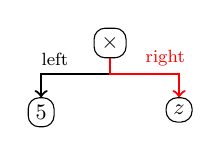
\begin{tikzpicture}[scale=0.8, every node/.style={scale=0.8}]
					\node (Times1) [stdNode] {
						$\times$
					};
					\node (cons1) [stdNode, below left = 2em of Times1] {
						5
					};
					\node (var1) [stdNode, below right = 2em of Times1] {
						$z$
					};
					\draw[thickarrow] (Times1.south)  -- ++(0,-0.25) -| (cons1.north) node [pos = 0.4, above, font=\footnotesize]{left};
					\draw[neglected] (Times1.south)  -- ++(0,-0.25) -| (var1.north) node [pos = 0.4, above, font=\footnotesize]{right};
					\end{tikzpicture}
				\end{figure}
			\end{exampleblock}
		\end{column}
	\end{columns}
	\begin{exampleblock}{Beispiel: query=$a$, Result=3}
		\begin{figure}[H]
			\centering
			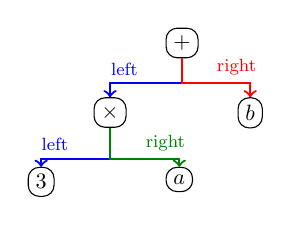
\begin{tikzpicture}[scale=0.8, every node/.style={scale=0.8}]
			\node (Plus) at (0,0) [stdNode] {
				$+$
			};
			\node (Times1) [stdNode, below left = 2em of Plus] {
				$\times$
			};
			\node (cons1) [stdNode, below left = 2em of Times1] {
				3
			};
			\node (var1) [stdNode, below right = 2em of Times1] {
				$a$
			};
			\node (var2) [stdNode, below right = 2em of Plus] {
				$b$
			};
			\draw[considered] (Plus.south)  -- ++(0,-0.4) -| (Times1.north) node [pos = 0.4, above, font=\footnotesize]{left};
			\draw[neglected] (Plus.south)  -- ++(0,-0.4) -| (var2.north) node [pos = 0.4, above, font=\footnotesize]{right};
			\draw[considered] (Times1.south)  -- ++(0,-0.5) -| (cons1.north) node [pos = 0.4, above, font=\footnotesize]{left};
			\draw[query] (Times1.south)  -- ++(0,-0.5) -| (var1.north) node [pos = 0.4, above, font=\footnotesize]{right};
			\end{tikzpicture}
		\end{figure}
	\end{exampleblock}
\end{frame}


\subsection{Herleitung: Iteration-Matrix \& Konstanten}
\begin{frame} % iterationmatrix
	\frametitle{\color{white}Iteration-Matrix \& Konstanten}
	\begin{itemize}
		\item Koeffizient f\"ur jede Variable und Konstante pro Update
		\item[$\Rightarrow$] Update-Matrix \& Konstanten \checkmark
		\uncover<2>{\item Iteration-Matrix \& Konstanten gegeben durch: 
			\begin{figure}[H]
				\centering
				$A = \begin{pmatrix} G & \textbf{0} \\ M & -I \\ -M & I \end{pmatrix}$ und $b = \begin{pmatrix} g \\ -u \\ u \end{pmatrix}$
			\end{figure}
		 k\"onnen berechnet werden
		 \item[$\Rightarrow$] Iteration-Matrix \& Konstanten \checkmark}
	\end{itemize}
\end{frame}

\subsection{Herleitung: SMT-Problem}
\begin{frame}
	\frametitle{SMT-Problem}
	\begin{itemize}
		\item Geg. Iteration-Matrix A und Iteration-Konstante b
		\item nutze SMT-Solver zum Beweis der (Nicht-)Existenz
		\item \red{Problem}: Teile des Ray-Kriteriums nicht linear
		\uncover<2>{\item[] zwei m\"ogliche L\"osungsans\"atze:
			\begin{enumerate}
				\item nutze \qfnia
				\item iteriere \"uber Unbekannte
			\end{enumerate}}
	\end{itemize}
\end{frame}

\begin{frame}
	\begin{variableblock}{Erinnerung: }{bg=orange!50!white,fg=black}{bg=orange, fg=white}
		\begin{itemize}
			\setlength{\itemindent}{1cm}
			\item[(domain)] $x, y_1, \dots, y_k \in \mathbb{R}^n$, $\lambda_1, \dots \lambda_k, \mu_1, \dots \mu_{k-1} \ge 0$
		\end{itemize}
	\end{variableblock}
	\begin{itemize}
		\item[] $\Rightarrow$ Bedingungen f\"ur  $\lambda_i$ und $\mu_i$ hinzuf\"ugen
	\end{itemize}
	\uncover<2>{\begin{variableblock}{Erinnerung:}{bg=orange!50!white,fg=black}{bg=orange, fg=white}
		\begin{itemize}
			\setlength{\itemindent}{1cm}
			\item[(init)] x repr\"asentiert den \stem
		\end{itemize}
	\end{variableblock}
	\begin{itemize}
		\item[] $\Rightarrow$ keine weiteren Bedingungen
	\end{itemize}}
	
\end{frame}

\begin{frame}
	\begin{variableblock}{Erinnerung: }{bg=orange!50!white,fg=black}{bg=orange, fg=white}
		\begin{itemize}
			\setlength{\itemindent}{1cm}
			\item[(point)] $A\begin{pmatrix} x \\ x + \sum_i y_i \end{pmatrix} \le b$
		\end{itemize}
	\end{variableblock}

	\begin{figure}[H]
		\centering		
		\only<1>{$\begin{pmatrix}G 	& \textbf{0} \\	U	& -I \\	-U & I \\\end{pmatrix} 
			\begin{pmatrix}	x \\ s \end{pmatrix} \le
			\begin{pmatrix}	g\\	-u\\ u\\ \end{pmatrix}$}
		\only<2>{$\begin{pmatrix}\blue{G} 	& \red{\textbf{0}} \\	U	& -I \\	-U & I \\\end{pmatrix} 
			\begin{pmatrix}	\blue{x} \\ \red{s} \end{pmatrix} \le
			\begin{pmatrix}	\blue{g}\\	-u\\ u\\ \end{pmatrix}$}
		\only<3>{$\begin{pmatrix}G 	& \textbf{0} \\	\blue{U}	& \blue{-I} \\	\red{-U} & \red{I} \\\end{pmatrix} 
			\begin{pmatrix}	x \\ s \end{pmatrix} \le
			\begin{pmatrix}	g\\	\blue{-u}\\ \red{u}\\ \end{pmatrix}$}
	\end{figure}
	
	\begin{itemize}
		\item[$\Rightarrow$]<2-> pr\"ufe Guard-Bedingungen f\"ur den \stem
		\item[]<3> eine Bedingung pro $s_i$ und
		\item[]<3> $n$ Bedingungen mit Gleichheit
		
	\end{itemize}
\end{frame}

\begin{frame}
	\begin{variableblock}{Erinnerung: Hergeleitete Matrix und Werte}{bg=orange!50!white,fg=black}{bg=orange, fg=white}
		\centering
		\begin{tabular}{rll}
			\multirow{2}{*}{$\begin{pmatrix}
				-1 		& -1 		&  0		& 0		 \\
				-1 		& 0 		&  0		& 0		 \\
				-3 		& 0 		&  0		& 0		 \\
				0 		& 2 		&  0		& 0		 \\
				3 		& 1 		&  -1		& 0		 \\
				0 		& 2 		&  0		& -1	 \\
				-3 		& -1 		&  1		& 0		 \\
				0 		& -2 		&  0		& 1	 	 \\
				\end{pmatrix}$}& &\multirow{2}{*}{$ \le \begin{pmatrix}
				-4 \\ -7 \\ -21 \\ -6 \\ 0 \\ 5 \\ 0 \\ -5
				\end{pmatrix} $}\\
			& & \\
			& \multirow{2}{*}{$\begin{pmatrix}
				x_{1,1} \\ x_{1,2} \\ s_{1} \\ s_{2}
				\end{pmatrix} $} & \\
			& & \\
			& & \\
			& & \\
			& & \\
			& & \\
		\end{tabular}
	\end{variableblock}
	\vspace*{-.5em}
	\begin{exampleblock}{Beispiel: Point Kriterium ($x=(10, -3)^T$ )}
		\begin{itemize}
			\item Guards: $-10-(-3)\le-4$
			\item Gleichheitsbedingung: $30-3-s_1=0$
			\item Summenbedingungen: $s_1= x_1+y_{1,1}+y_{2,1}$ und $s_2=x_2+y_{1,2}+y_{2,2}$
		\end{itemize}
	\end{exampleblock}	
\end{frame}

\begin{frame}
	\begin{variableblock}{Erinnerung: Ray Kriterium}{bg=orange!50!white,fg=black}{bg=orange, fg=white}
		\begin{itemize}
			\setlength{\itemindent}{1cm}
			\item[(ray)] $A\begin{pmatrix} y_i \\ \lambda_i y_i + \mu_{i-1} y_{i-1} \end{pmatrix} \le 0$ for all $1 \le i \le k$
		\end{itemize}
	\end{variableblock}
	F\"uge Bedingungen hinzu:
	\begin{itemize}
		\setlength{\itemindent}{1cm}
		\item[$i=1$:] $\Rightarrow \mu_{i-1}y_{i-1}=0 \Rightarrow $ $A\begin{pmatrix} y_1 \\ \lambda_1 y_1 \end{pmatrix} \le 0$
		\item[$i>1$:] mit $\lambda_i$ als den $i$-ten Eigenwert
		\item[]
		\item[] $\Rightarrow$ alle n\"otigen Bedingungen  hinzugef\"ugt\checkmark
		\item[] lasse den \solver ein GNA herleiten
	\end{itemize}	
\end{frame}

\begin{frame}
	\begin{variableblock}{Erinnerung: Hergeleitete Matrix und Werte}{bg=orange!50!white,fg=black}{bg=orange, fg=white}
	\begin{tabular}{rll}
		\multirow{2}{*}{$\begin{pmatrix}
			-1 		& -1 		&  0		& 0		 \\
			-1 		& 0 		&  0		& 0		 \\
			-3 		& 0 		&  0		& 0		 \\
			0 		& 2 		&  0		& 0		 \\
			3 		& 1 		&  -1		& 0		 \\
			0 		& 2 		&  0		& -1	 \\
			-3 		& -1 		&  1		& 0		 \\
			0 		& -2 		&  0		& 1	 	 \\
			\end{pmatrix}$}& &\multirow{2}{*}{$ \le \begin{pmatrix}
			0 \\ 0 \\ 0 \\ 0 \\ 0 \\ 0 \\ 0 \\ 0 \\ 
			\end{pmatrix} $}\\
		& & \\
		& \multirow{2}{*}{$\begin{pmatrix}
			y_{i,1} \\ y_{i,2} \\ \lambda_iy_{i,1}+\mu_{i-1}y_{i-1,1} \\ \lambda_iy_{i,2}+\mu_{i-1}y_{i-1,2}
			\end{pmatrix} $} & \\
		& & \\
		& & \\
		& & \\
		& & \\
		& & \\
	\end{tabular}
	\end{variableblock}
	\vspace*{-.5em}
	\begin{exampleblock}{Beispiel: Ray Kriterium ($\lambda_1 = 3,\lambda_2 = 2$) }
		\begin{itemize}
			\setlength{\itemindent}{0.25cm}
			\item[i=1:] Beispielbedingung: $-y_{1,1}-y_{1,2} \le -4$, $3\cdot y_{1,1}+y_{1,2}-3\cdot y_{1,1}=0$
			\item[i$=$2:] Beispielbedingung: $-y_{2,1}-y_{2,2} \le -4$, 
			\item[] $3\cdot y_{2,1}+y_{2,2}-1\cdot (2\cdot y_{2,1}+\mu\cdot y_{1,1})=0$
		\end{itemize}
	\end{exampleblock}
\end{frame}




\section{Beispiel  eines GNAs}
\frame{\tableofcontents[currentsection]}
\begin{frame}
	\frametitle{\color{white}Beispiel  eines GNAs}
	\begin{exampleblock}{Beispiel eines GNAs \rom{1}}
		Vom \solver: $y_1=\begin{pmatrix} 9 \\ 0 \end{pmatrix}$, $y_2=\begin{pmatrix} 8 \\ -8 \end{pmatrix}$, $\mu_1=0$\newline
		\vspace*{-.8em}
		\begin{itemize}
			\setlength{\itemindent}{1.5cm}
			\item[(domain)] offensichtlich wahr \checkmark
			\item[(init)] Berechnung des \stem (\checkmark)
			\item[(point)]  $A\begin{pmatrix} 10 \\ -3 \\ 10+9+8 \\ -3 + 0 + (-8) \end{pmatrix} \le b \Leftrightarrow A\begin{pmatrix} 10 \\ -3 \\ 27 \\ -11 \end{pmatrix} \le b$ \checkmark
		\end{itemize}
	\end{exampleblock}
\end{frame}

\begin{frame}
	\begin{exampleblock}{Beispiel eines GNAs \rom{2}}
		Vom \solver: $y_1=\begin{pmatrix} 9 \\ 0 \end{pmatrix}$, $y_2=\begin{pmatrix} 8 \\ -8 \end{pmatrix}$, $\mu_1=0$\newline
		\begin{itemize}
			\setlength{\itemindent}{0.5cm}
			\item[(ray)]
			\item[$i=1$:]  $A\begin{pmatrix} 9 \\ 0 \\ 3\cdot 9 \\ 3\cdot 0 \end{pmatrix} \le 0 \Leftrightarrow A\begin{pmatrix} 9 \\ 0 \\ 27 \\ 0 \end{pmatrix} \le 0$ \checkmark
			\item[$i>1$:] $A\begin{pmatrix} 8 \\ -8 \\ 2\cdot 8+0\cdot 9 \\ 2\cdot (-8)+0\cdot 0 \end{pmatrix} \le 0 \Leftrightarrow A\begin{pmatrix} 8 \\ -8 \\ 16 \\ -16 \end{pmatrix} \le 0$ \checkmark
		\end{itemize}
		$\Rightarrow$ das GNA erf\"ullt alle Kriterien\newline
		$\Rightarrow$ Nichtterminierung ist bewiesen
	\end{exampleblock}
\end{frame}







\end{document}